%%%%%%%%%%%%%%%%%%%%%%%%%%%%%%%%%%%%%%%%%
% Beamer Presentation
% LaTeX Template
% Version 1.0 (10/11/12)
%
% This template has been downloaded from:
% http://www.LaTeXTemplates.com
%
% License:
% CC BY-NC-SA 3.0 (http://creativecommons.org/licenses/by-nc-sa/3.0/)
%
%%%%%%%%%%%%%%%%%%%%%%%%%%%%%%%%%%%%%%%%%

%----------------------------------------------------------------------------------------
%	PACKAGES AND THEMES
%----------------------------------------------------------------------------------------

\documentclass{beamer}

\mode<presentation> {

% The Beamer class comes with a number of default slide themes
% which change the colors and layouts of slides. Below this is a list
% of all the themes, uncomment each in turn to see what they look like.

%\usetheme{default}
%\usetheme{AnnArbor}
%\usetheme{Antibes}
%\usetheme{Bergen}
%\usetheme{Berkeley}
%\usetheme{Berlin}
%\usetheme{Boadilla}
%\usetheme{CambridgeUS}
%\usetheme{Copenhagen}
%\usetheme{Darmstadt}
%\usetheme{Dresden}
%\usetheme{Frankfurt}
%\usetheme{Goettingen}
%\usetheme{Hannover}
%\usetheme{Ilmenau}
%\usetheme{JuanLesPins}
%\usetheme{Luebeck}
\usetheme{Madrid}
%\usetheme{Malmoe}
%\usetheme{Marburg}
%\usetheme{Montpellier}
%\usetheme{PaloAlto}
%\usetheme{Pittsburgh}
%\usetheme{Rochester}
%\usetheme{Singapore}
%\usetheme{Szeged}
%\usetheme{Warsaw}

% As well as themes, the Beamer class has a number of color themes
% for any slide theme. Uncomment each of these in turn to see how it
% changes the colors of your current slide theme.

%\usecolortheme{albatross}
\usecolortheme{beaver}
%\usecolortheme{beetle}
%\usecolortheme{crane}
%\usecolortheme{dolphin}
%\usecolortheme{dove}
%\usecolortheme{fly}
%\usecolortheme{lily}
%\usecolortheme{orchid}
%\usecolortheme{rose}
%\usecolortheme{seagull}
%\usecolortheme{seahorse}
%\usecolortheme{whale}
%\usecolortheme{wolverine}

%\setbeamertemplate{footline} % To remove the footer line in all slides uncomment this line
%\setbeamertemplate{footline}[page number] % To replace the footer line in all slides with a simple slide count uncomment this line

%\setbeamertemplate{navigation symbols}{} % To remove the navigation symbols from the bottom of all slides uncomment this line
}

\usepackage{graphicx} % Allows including images
\usepackage{booktabs} % Allows the use of \toprule, \midrule and \bottomrule in tables
\usepackage{tcolorbox}
\usepackage{tikz}
\usetikzlibrary{shapes.arrows}
\usepackage[absolute,overlay]{textpos}
  \setlength{\TPHorizModule}{1mm}
  \setlength{\TPVertModule}{1mm}

\addtobeamertemplate{frametitle}{}{%
\begin{textblock*}{100mm}(.85\textwidth,-0.25cm)

\includegraphics[scale=0.25]{logo.png}
\end{textblock*}}

%----------------------------------------------------------------------------------------
%	GRAPHICS PATH
%----------------------------------------------------------------------------------------
\graphicspath{{./fig/}}

%----------------------------------------------------------------------------------------
%	TITLE PAGE
%----------------------------------------------------------------------------------------

\title[PRT551 - Lecture 3]{Project Management, Risk, and Reliability} % The short title appears at the bottom of every slide, the full title is only on the title page

\author{Associate Professor Sureshkumar} % Your name
\institute[CDU] % Your institution as it will appear on the bottom of every slide, may be shorthand to save space
{
Charles Darwin University \\ % Your institution for the title page
\medskip
\textit{cdux@cdu.edu.au} % Your email address
}
\date{\today} % Date, can be changed to a custom date

\begin{document}

\begin{frame}
\titlepage % Print the title page as the first slide
\begin{textblock}{20}(80,30)
      
\includegraphics[scale=0.8]{logo_1.png}
\end{textblock}
\end{frame}

%---------------------------------------------------------
%	PRESENTATION SLIDES
%---------------------------------------------------------


%---------------------------------------------------------

\begin{frame}
\frametitle{Learning Objectives}
\begin{itemize}
\item Describe the five project management process groups, map them to the project management knowledge areas, discuss why organizations develop their own project management methodologies, and understand the importance of top management commitment and organizational standards in project management;
\item Discuss the initiating process, including pre-initiating tasks, breaking large projects down into smaller projects, and initiating tasks;
\item Identify project stakeholders and perform a stakeholder analysis;
\item Prepare a business case to justify the need for a project;
\item Create a project charter to formally initiate a project;
\item Describe the importance of holding a good project kick-off meeting;
\item Develop a preliminary project scope statement to help understand project requirements.
\end{itemize}

\end{frame}

%---------------------------------------------------------
\begin{frame}
\frametitle{The Importance of Top Management Commitment}
\vspace{-0.1cm}
\begin{itemize}
\item Without top management, many projects will fail.
\item Some projects have a senior manager called a \textbf{champion} who acts as a key proponent for a project.
\item Projects are part of the larger organisational environment, and many factors are out of the project manager's control.
\end{itemize}

\begin{tcolorbox}
\textbf{How Top Managers Help Project Managers Succeed}
\footnotesize
\begin{itemize}
\item Provide adequate resources
\item Timely approval on unique needs
\item Deal with other departments
\item Deal with 'politics'
\item Leadership development
\item Develop and enforce organisational standards
\item Support project management office (PMO)
\end{itemize}
\end{tcolorbox}
\end{frame}

%---------------------------------------------------------
\begin{frame}
\frametitle{Project Management Office (PMO)}
\begin{block}{Definition: \textbf{Project Management Office (PMO)}}
A \textbf{project management office (PMO)} is an organisational entity created to assist project managers in achieving project goals.
\end{block}
\vspace{0.2cm}
A \textbf{PMO} can help development standards and methodologies standards and methodologies, provide career paths for project managers, and assist project managers with training and certification.
\begin{figure}
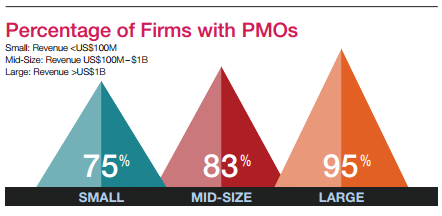
\includegraphics[scale=0.4]{PMO}
\caption{Source: "The State of the PMO 2016"}
\end{figure}
\end{frame}

%---------------------------------------------------------
\begin{frame}
\frametitle{Project Management Office (PMO)}
\textbf{Possible Goals of a PMO}
\vspace{0.5cm}
\begin{itemize}
\item Collect, organise, and integrate project data for the entire organisation;
\item Research, develop, and share best practices in project management;
\item Develop and maintain templates, tools, standards, and methodologies;
\item Develop and provide a formal career path for project managers;
\item Provide project management consulting services;
\item Provide a structure to house project managers while then are acting in those roles or are between projects.
\end{itemize}
\end{frame}

%---------------------------------------------------------
\begin{frame}
\frametitle{Developing a Project Management Methodology}
\begin{block}{Definition: \textbf{Methodology}}
A \textbf{methodology} describes how things should be done.
\end{block}
\begin{itemize}
\item The \textit{PMBOK Guide} is a methodology  and a \textbf{standard} that describes best practices for what should be done to manage a project.
\item Another project management methodology is \textbf{PRojects IN Controlled Environments (PRINCE2)}. This was originally developed for IT projects and was released in 1996 by the U.K. Office of Government.
\item \textbf{Agile} is yet another project management methodology which is used by many software development projects. This methodology focuses on iterative workflow and incremental delivery of software in short iterations.
\end{itemize}
\end{frame}

%---------------------------------------------------------
\begin{frame}
\frametitle{Developing a Project Management Methodology}
\textbf{Agile Project Management}
\vspace{0.5cm}
\begin{block}{Definition: \textbf{Agile}}
Relating to or denoting a method of project management used especially for software development, that is characterised by the division of tasks into short phases of work and frequent reassessment and adaptation of plans.
\end{block}
\begin{itemize}
\item Early software development projects used a waterfall approach, where requirements were defined in detail before any software was written.
\item As the rate of change of business technology increased, this approach became unrealistic for many projects.
\end{itemize}
\end{frame}

%---------------------------------------------------------
\begin{frame}
\frametitle{Developing a Project Management Methodology}
\textbf{Scrum}
\vspace{0.25cm}
\begin{itemize}
\item \textbf{Scrum} is the leading agile development method for completing projects with a complex, innovative scope of work.
\item The term was coined in 1986 in a Harvard Business Review study that compared high-performing, cross-functional teams to the scrum formation used by rugby teams.
\end{itemize}
\begin{figure}
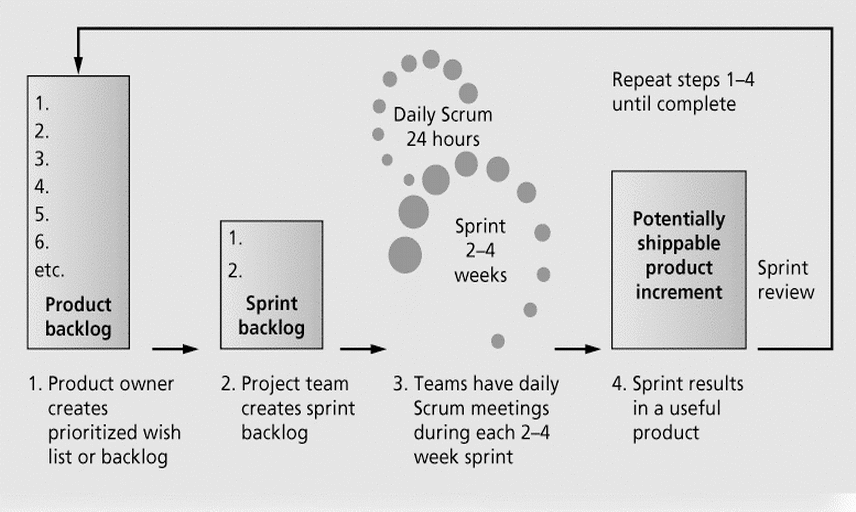
\includegraphics[scale=0.27]{scrum}
\caption{The figure shows the scrum framework}
\end{figure}
\end{frame}

%---------------------------------------------------------
\begin{frame}
\frametitle{Developing a Project Management Methodology}
The project management methodology that this course will be focused on is the \textit{PMBOK}, shown below.
\begin{figure}
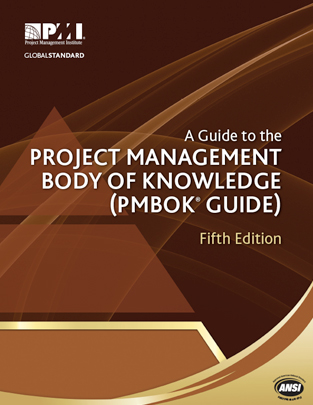
\includegraphics[scale=0.3]{pmbok_guide}
\caption{PMBOK stands for project management body of knowledge, and is the project management methodology.}
\end{figure}
\end{frame}
%---------------------------------------------------------

\begin{frame}
\frametitle{Project Management Process Groups}
\begin{block}{Definition: \textbf{Process}}
A \textbf{process} is a series of actions directed towards a particular result
\end{block}
\vspace{0.5cm}
\begin{block}{Definition: \textbf{Process Groups}}
Project management \textbf{process groups} progress from initiating activities to planning activities, executing activities, monitoring and controlling activities, and closing activities.
\end{block}

\end{frame}

%----------------------------------------------------------

\begin{frame}
\frametitle{Description of Process Groups}
\begin{itemize}
\item \textbf{Initiating processes}: include actions to begin projects and project phases
\item \textbf{Planning processes}: include devising and maintaining a workable scheme to ensure that the project meets its scope, time, and cost goals as well as organisational needs
\item \textbf{Executing processes}: include coordinating people and other resources to carry out the project plans and produce the deliverables of the project or phase.
\item \textbf{Monitoring and controlling processes}: measure progress towards achieving project goals, monitor deviation from plans, and take corrective action to match progress with plans and customer expectations
\item \textbf{Closing processes}: include formalising acceptance of the project or phase and bringing it to an orderly end
\end{itemize}
\end{frame}

%---------------------------------------------------------
\begin{frame}
\frametitle{Project Management Process Groups}
The process groups have clear dependencies and are performed in the same sequence on each project.
\begin{figure}
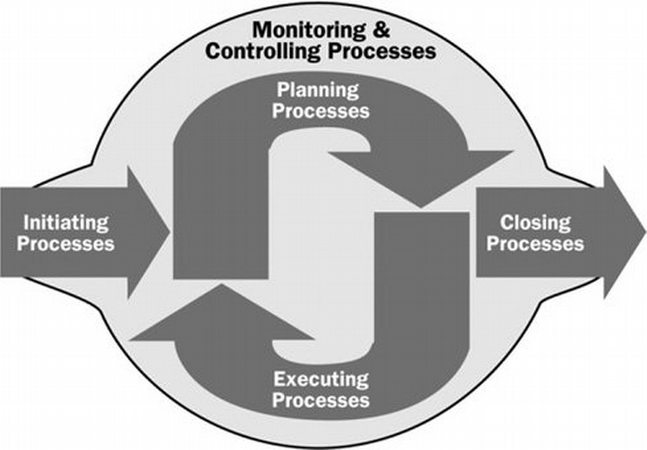
\includegraphics[scale=0.45]{process_seq}
\caption{The diagram helps to understand how the process groups are sequenced}
\end{figure}
\end{frame}

%----------------------------------------------------------
\begin{frame}
\frametitle{Characteristics of the Process Groups}
The level of activity and length of each process group varies for every project:
\begin{itemize}
\item Normally, executing tasks require the most resources and time, followed by planning tasks;
\item Monitoring and controlling processes are done throughout the project's lifespan;
\item Initiating and closing tasks are usually the shortest (at the beginning and end of a project or phase, respectively), and they require the least amount of resources and time.
\end{itemize}
Note that process groups apply to the entire project as well as to the project phases.
\begin{block}{Definition: \textbf{Phase}}
A \textbf{phase} is a distinct stage in project development, and most projects have distinct phases.
\end{block}
\end{frame}

%----------------------------------------------------------
\begin{frame}
\frametitle{Guidelines for Time Spent in Each Process Group}
\begin{figure}
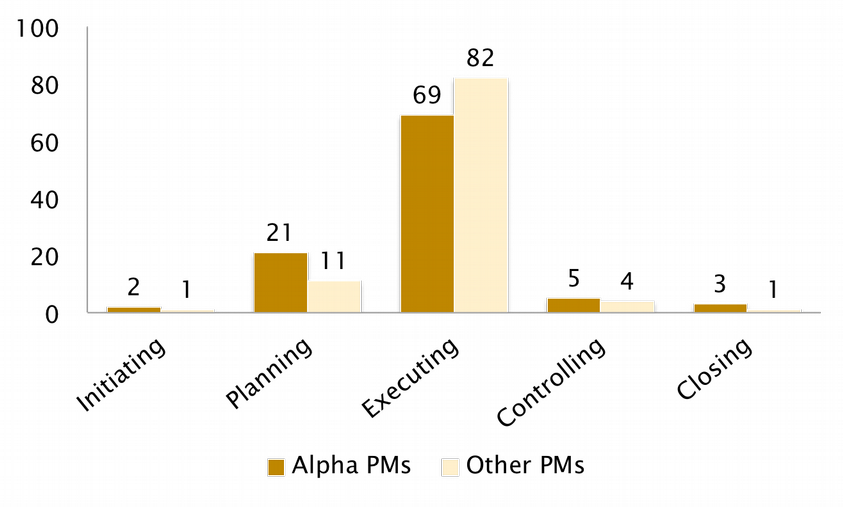
\includegraphics[scale=0.45]{time_spent_proc}
\caption{The graph shows the approximate percentage of the total time that a project will spend on each process group}
\end{figure}
\end{frame}

%----------------------------------------------------------
\begin{frame}
\frametitle{Mapping of Knowledge Area to Process Group}
\begin{figure}
\caption{This diagram will act as a map to the project management process - we will use it again and again to orient your learning of project management.}
\vspace{-0.8cm}
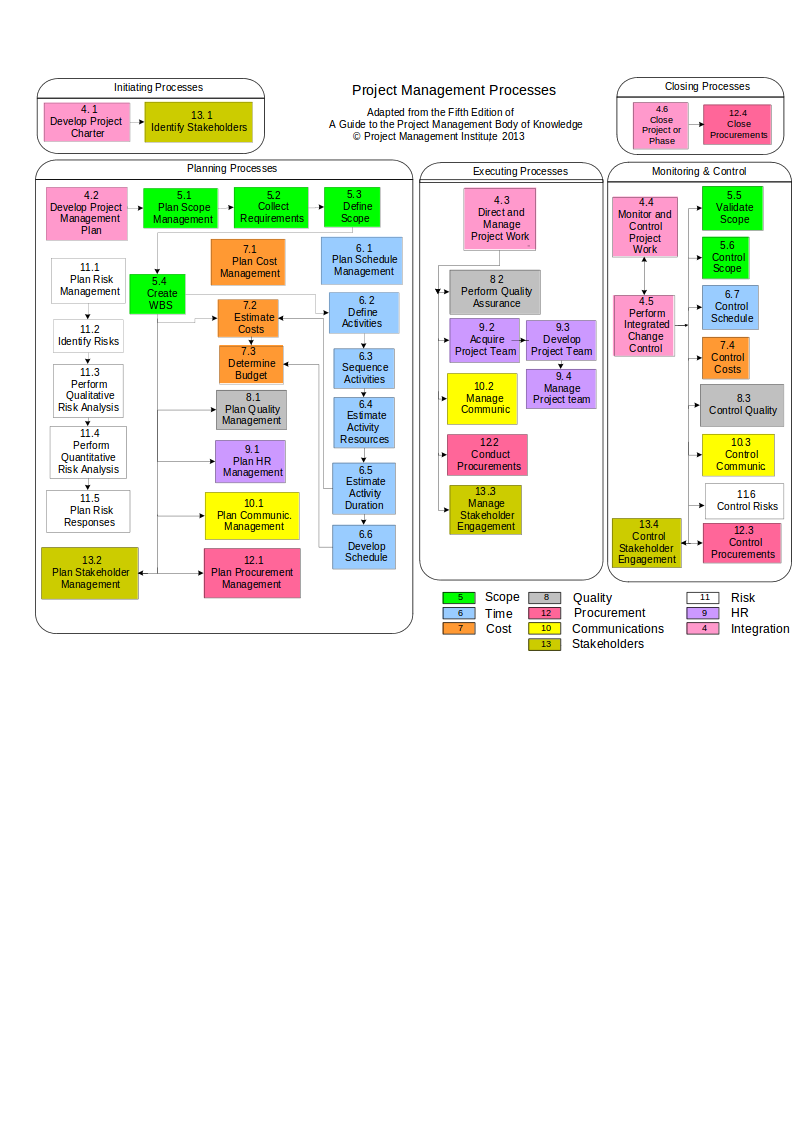
\includegraphics[scale=0.3]{mapping}
\end{figure}
\end{frame}

%----------------------------------------------------------
\begin{frame}
\frametitle{What Happens Prior to the Initiating Process?}
\begin{figure}
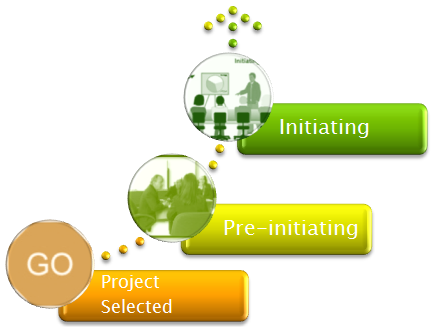
\includegraphics[scale=0.8]{init}
\end{figure}
\end{frame}

%----------------------------------------------------------
\begin{frame}
\frametitle{What Happens Prior to the Initiating Process?}
\begin{columns}
\column{0.43\textwidth}
\begin{tcolorbox}
\textbf{Pre-initiating}\\
\textbf{(Senior Management)}
\begin{itemize}
\item Identify scope, time, and cost;
\item Identify project sponsor;
\item Select project manager;
\item Develop \textbf{business case} for the project;
\item Review processes and expectations;
\end{itemize}
\end{tcolorbox}
\column{0.12\textwidth}
\begin{figure}
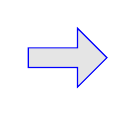
\begin{tikzpicture}
\node[single arrow,draw=blue,fill=black!10,minimum height=1cm,shape border rotate=0] at (0,0) {};
\end{tikzpicture}
\end{figure}
\column{0.43\textwidth}
\begin{tcolorbox}
\textbf{Initiating}\\
\textbf{(Project Manager)}
\begin{itemize}
\item Identify and understand all project stakeholders;
\item Develop project charter
\item Hold kick-off meeting
\item Preliminary scope statement
\end{itemize}
\end{tcolorbox}
\end{columns}
\end{frame}

%----------------------------------------------------------
\begin{frame}
\frametitle{What Happens Prior to the Initiating Process?}
\textbf{Pre-initiating Processes}\\
\vspace{0.5cm}
It is good practice to lay the groundwork for a project before it officially starts. After a project is approved, senior managers should meet to accomplish the following tasks:
\vspace{0.5cm}
\begin{itemize}
\item Determine the scope time, and cost \textbf{constraints} for the project;
\item Identify the \textbf{project sponsor};
\item Select the \textbf{project manager};
\item Meet with the project manager to review the process and expectations for managing the project;
\item Determine if the project should be divided into two or more smaller projects because it is easier to manage smaller projects than larger ones.
\end{itemize}
\end{frame}

%----------------------------------------------------------
\begin{frame}
\frametitle{What Happens Prior to the Initiating Process?}
\textbf{Business Case}\\
\vspace{0.5cm}
A \textbf{business case} is just a document that provides financial justification for investing in a project. Typically a \textbf{business case} will contain:
\begin{itemize}
\item Introduction and background
\item Business Objective
\item Current situation and problem/opportunity statement
\item Critical assumptions and constraints
\item Analysis of options and recommendation
\item Preliminary project requirements
\item Budget estimate and financial analysis
\item Schedule estimate
\item Potential risks
\end{itemize}
\end{frame}

%----------------------------------------------------------
\begin{frame}
\frametitle{What Happens Prior to the Initiating Process?}
\textbf{Business Case}\\
\vspace{0.2cm}
A business case is a standard document used by project managers. To get an idea of what a business case document looks like try Googling \textit{business case templates}.
\begin{figure}
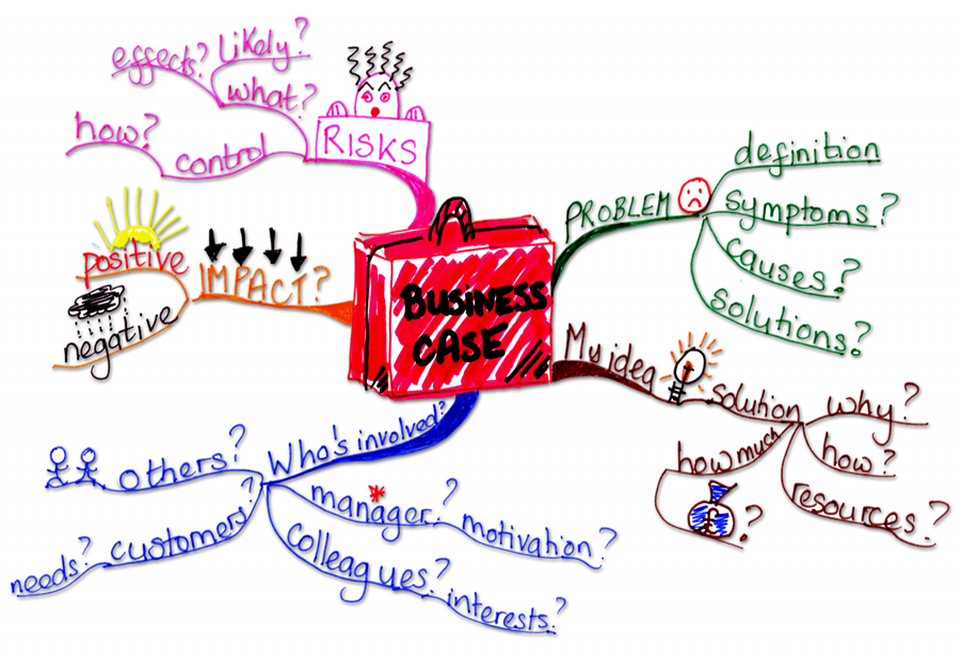
\includegraphics[scale=0.25]{bus_case}
\caption{An example of a mind map to help you generate ideas for your business case.}
\end{figure}
\end{frame}

%----------------------------------------------------------
\begin{frame}
\frametitle{Project Charter}
\begin{figure}
\caption{The task of developing a project charter is in the \textbf{Integration} knowledge area, and belongs to the \textbf{Initiating} process group.}
\vspace{-0.8cm}
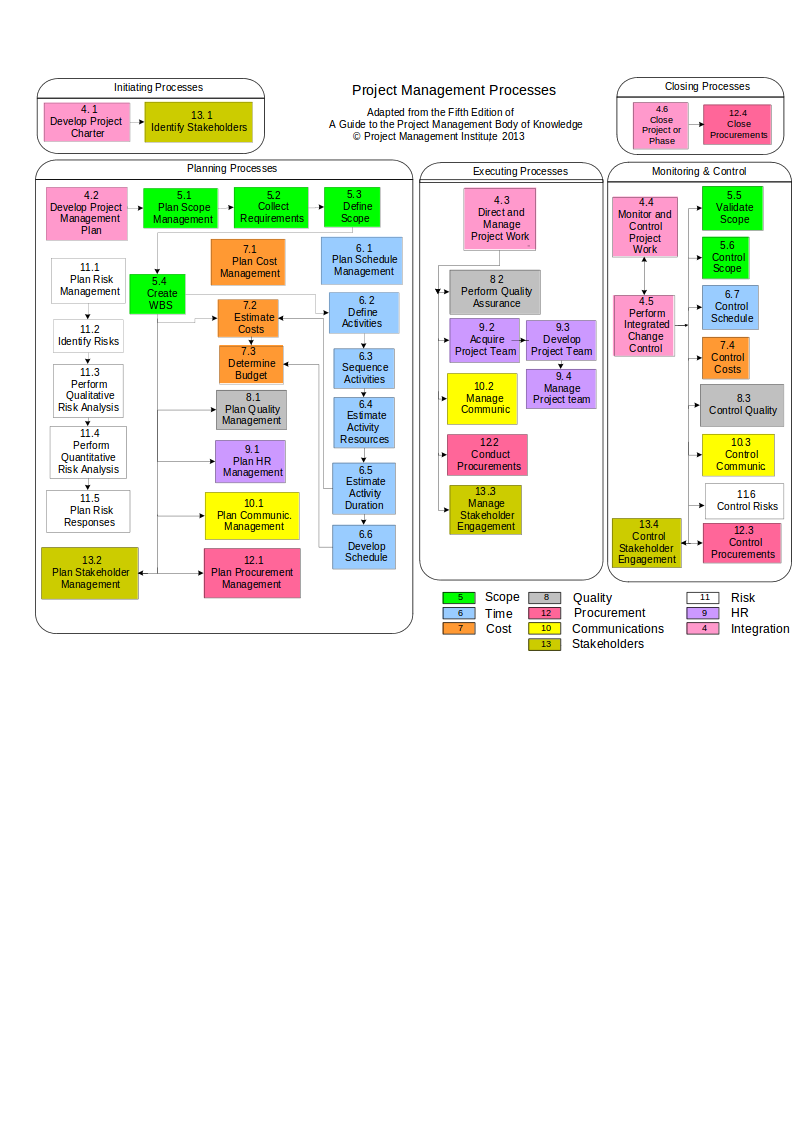
\includegraphics[scale=0.3]{mapping}
\end{figure}
\end{frame}

%----------------------------------------------------------
\begin{frame}
\frametitle{Project Charter}
\textbf{Creating a Project Charter}
\vspace{0.25cm}
\begin{block}{Definition: \textbf{Project Charter}}
A \textbf{project charter} is a document that formally recognises the existence of a project and provides a summary of the project's objectives and management
\end{block}
\vspace{0.25cm}
\begin{itemize}
\item A project charter authorises the project manager to use organisational resources to complete the project;
\item The project manager plays a major role in developing the project charter;
\item A crucial part of the project charter is the sign off section.
\item Instead of project charters, some organisations initiate projects using a simple letter of agreement or formal contracts
\end{itemize}
\end{frame}

%----------------------------------------------------------
\begin{frame}
\frametitle{Project Charter}
\textbf{Contents of a Project Charter}
\vspace{0.5cm}
\begin{itemize}
\item The project's title and date of authorisation;
\item The project manager's name and contact information;
\item A summary schedule or timeline, including the planned start and finish dates. If a summary milestone schedule is available, it should also be included or referenced;
\item A summary of the project's estimated cost and budget allocation;
\item A brief description of the project's objectives, including the business need or other justification for authorising the project;
\item Project success criteria, including project approval requirements and who signs off on the project.
\end{itemize}
\end{frame}

%----------------------------------------------------------
\begin{frame}
\frametitle{Project Charter}
\textbf{Contents of a Project Charter (Continued)}
\vspace{0.5cm}
\begin{itemize}
\item A summary of the planned approach for managing the project, which should describe stakeholder needs and expectations, important assumptions and constraints, and should refer to related documents, such as a communications management plan, as available;
\item A roles and responsibilities matrix;
\item A sign-off section for signatures of key project stakeholders;
\item A comments section in which stakeholders can provide important comments related to the project.
\end{itemize}
\end{frame}

%----------------------------------------------------------
\begin{frame}
\frametitle{Project Charter}
\textbf{Example of a Project Charter}
\vspace{-0.2cm}
\begin{columns}
\column{0.45\textwidth}
\begin{figure}
\frame{
\includegraphics[scale=0.23]{pg_1}}
\end{figure}
\column{0.5\textwidth}
\begin{figure}
\frame{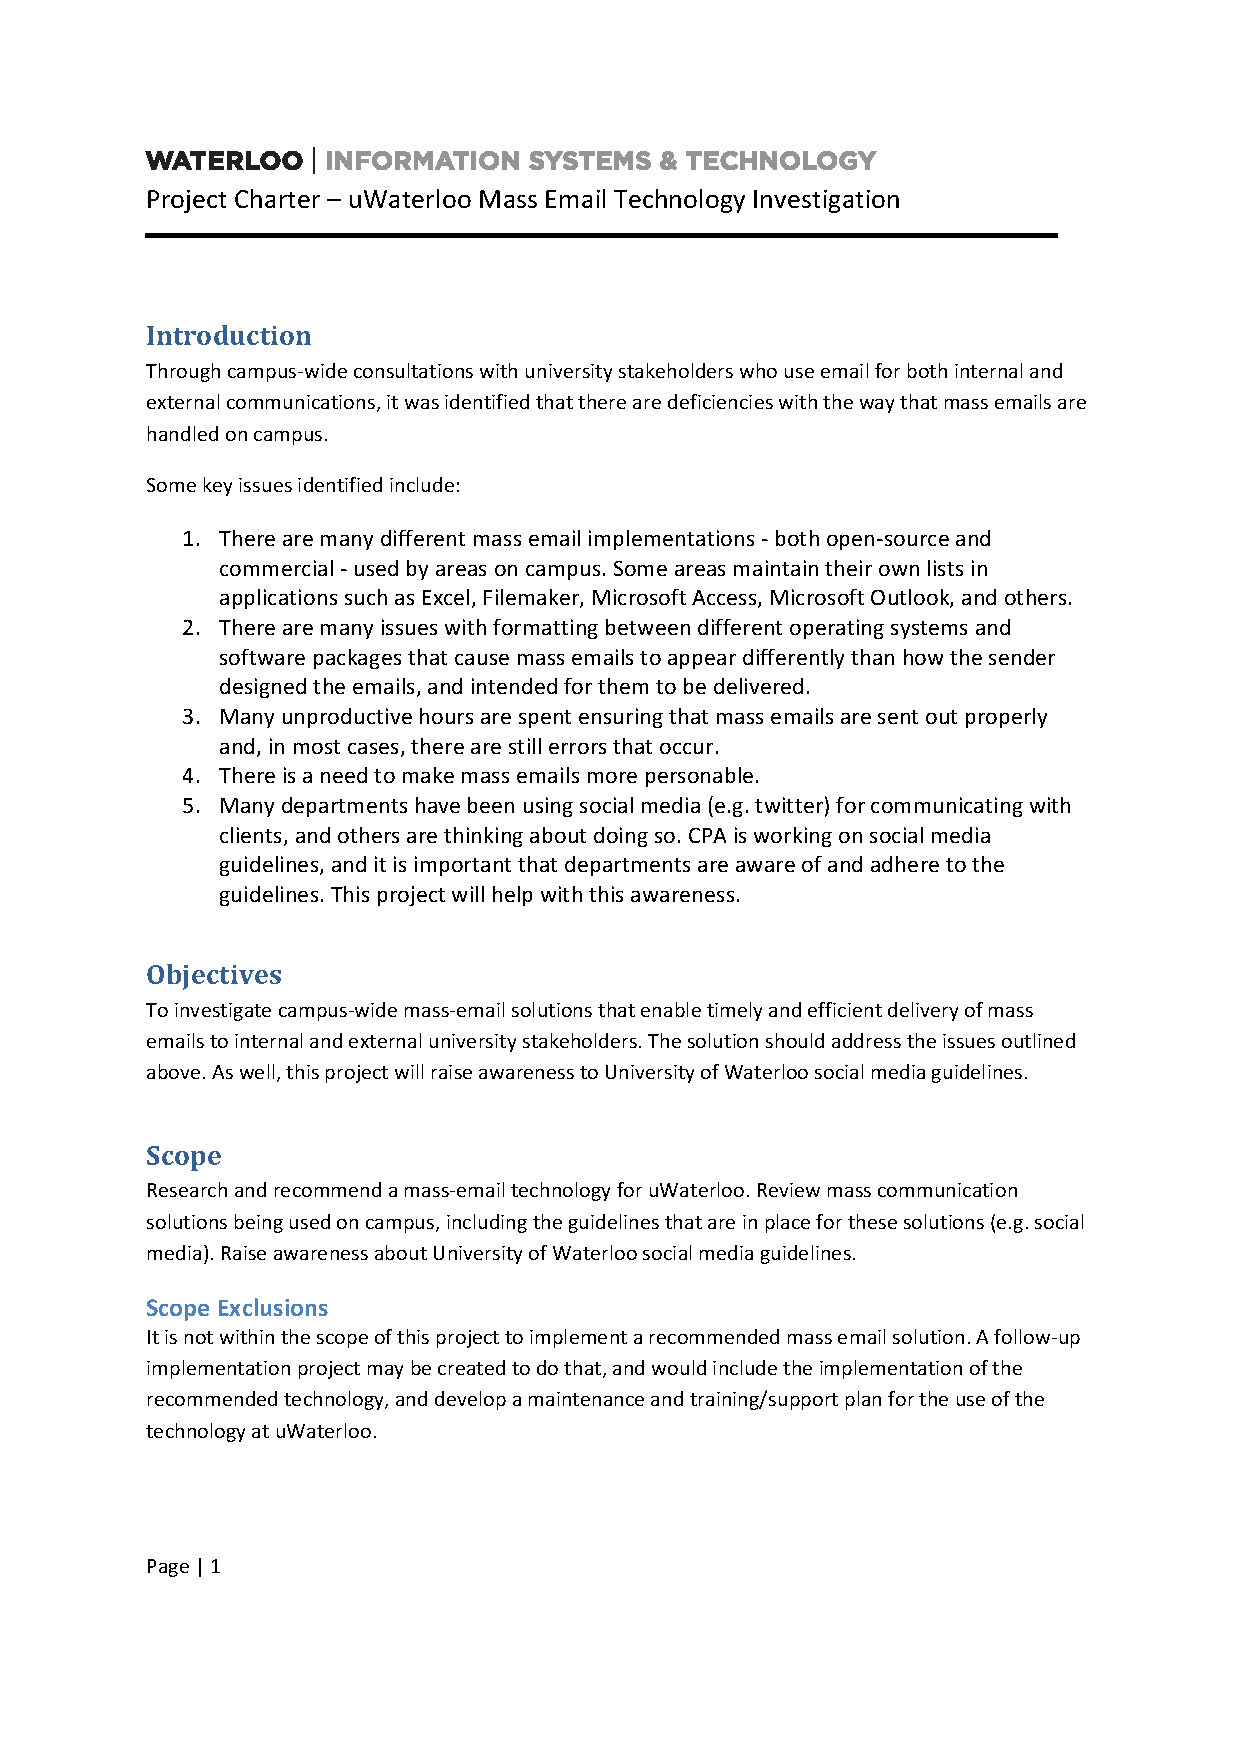
\includegraphics[scale=0.23]{pg_2}}
\end{figure}
\end{columns}
\end{frame}

%----------------------------------------------------------
\begin{frame}
\frametitle{Project Charter}
\textbf{Example of a Project Charter}
\vspace{-0.2cm}
\begin{columns}
\column{0.45\textwidth}
\begin{figure}
\frame{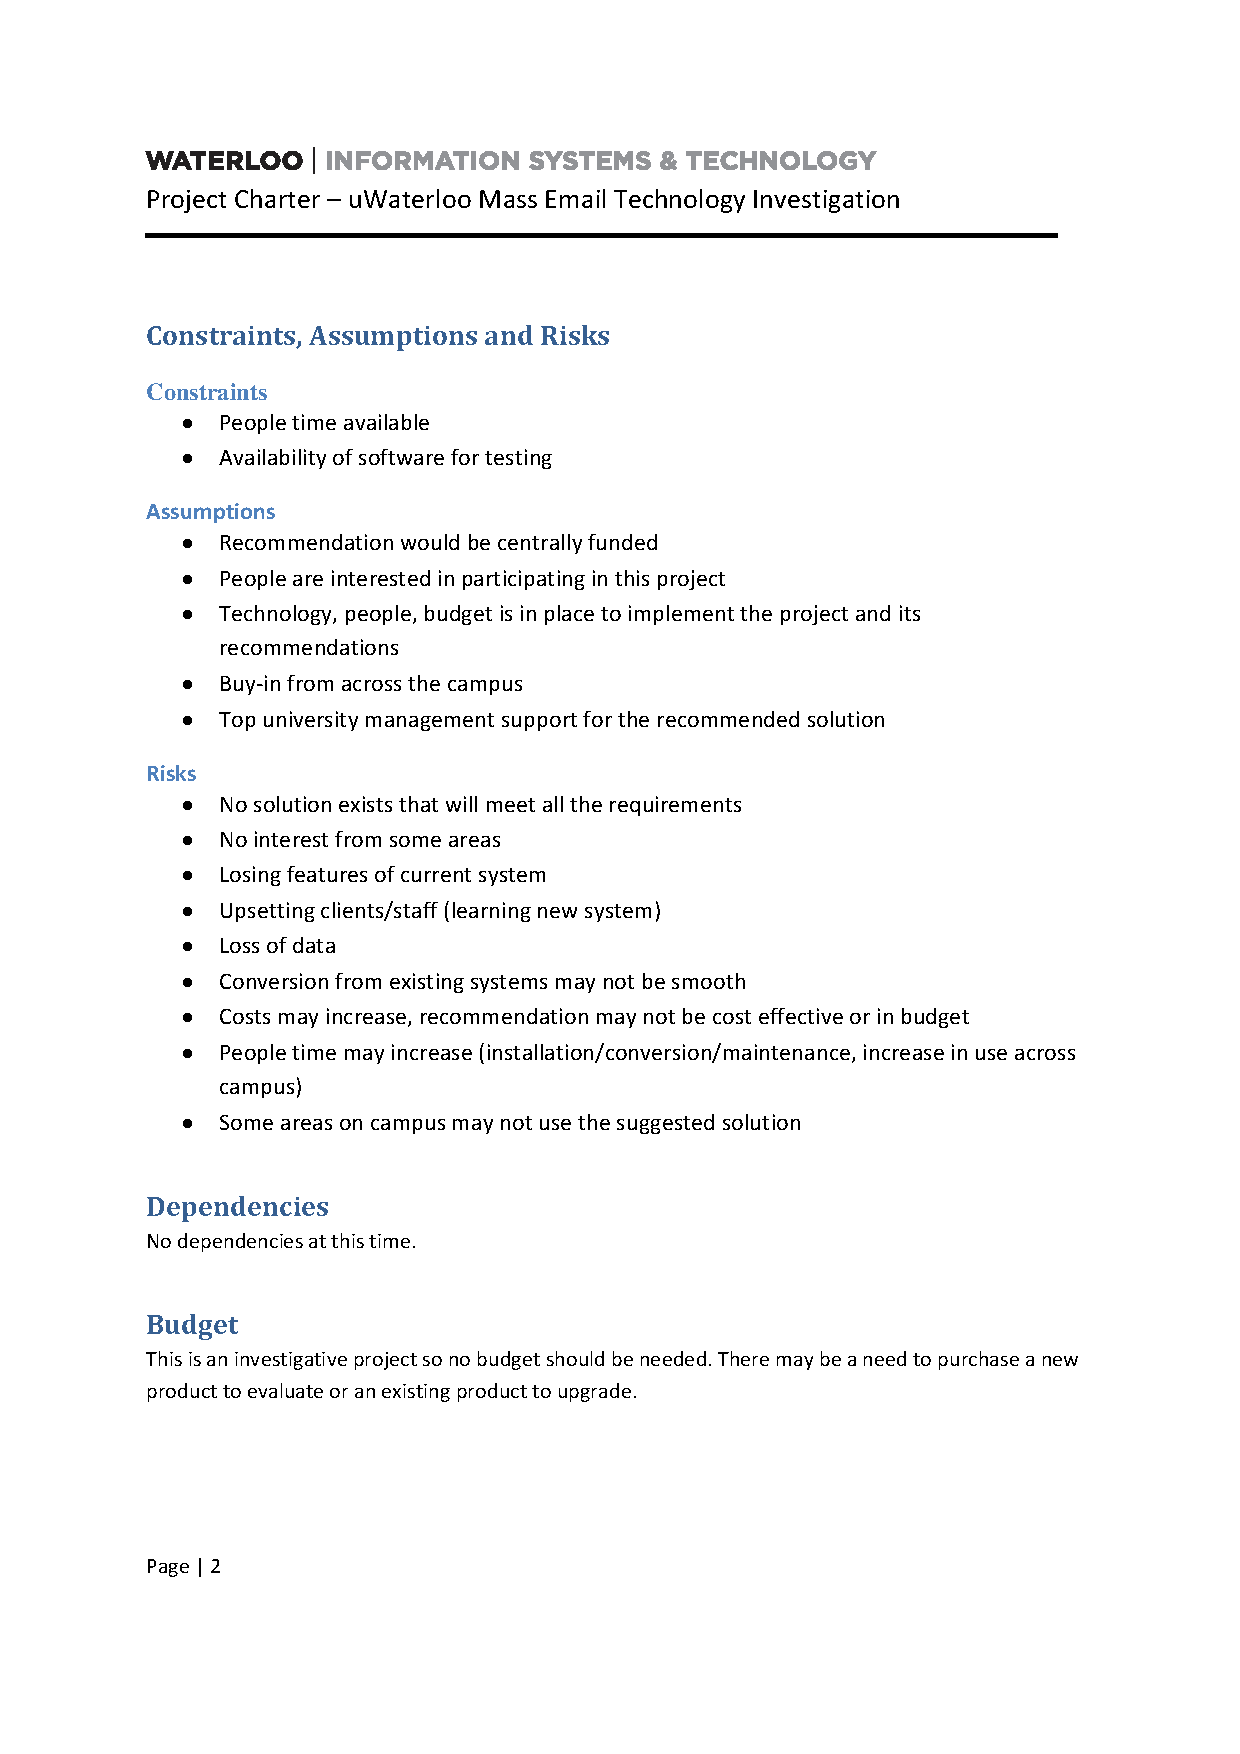
\includegraphics[scale=0.23]{pg_3}}
\end{figure}
\column{0.5\textwidth}
\begin{figure}
\frame{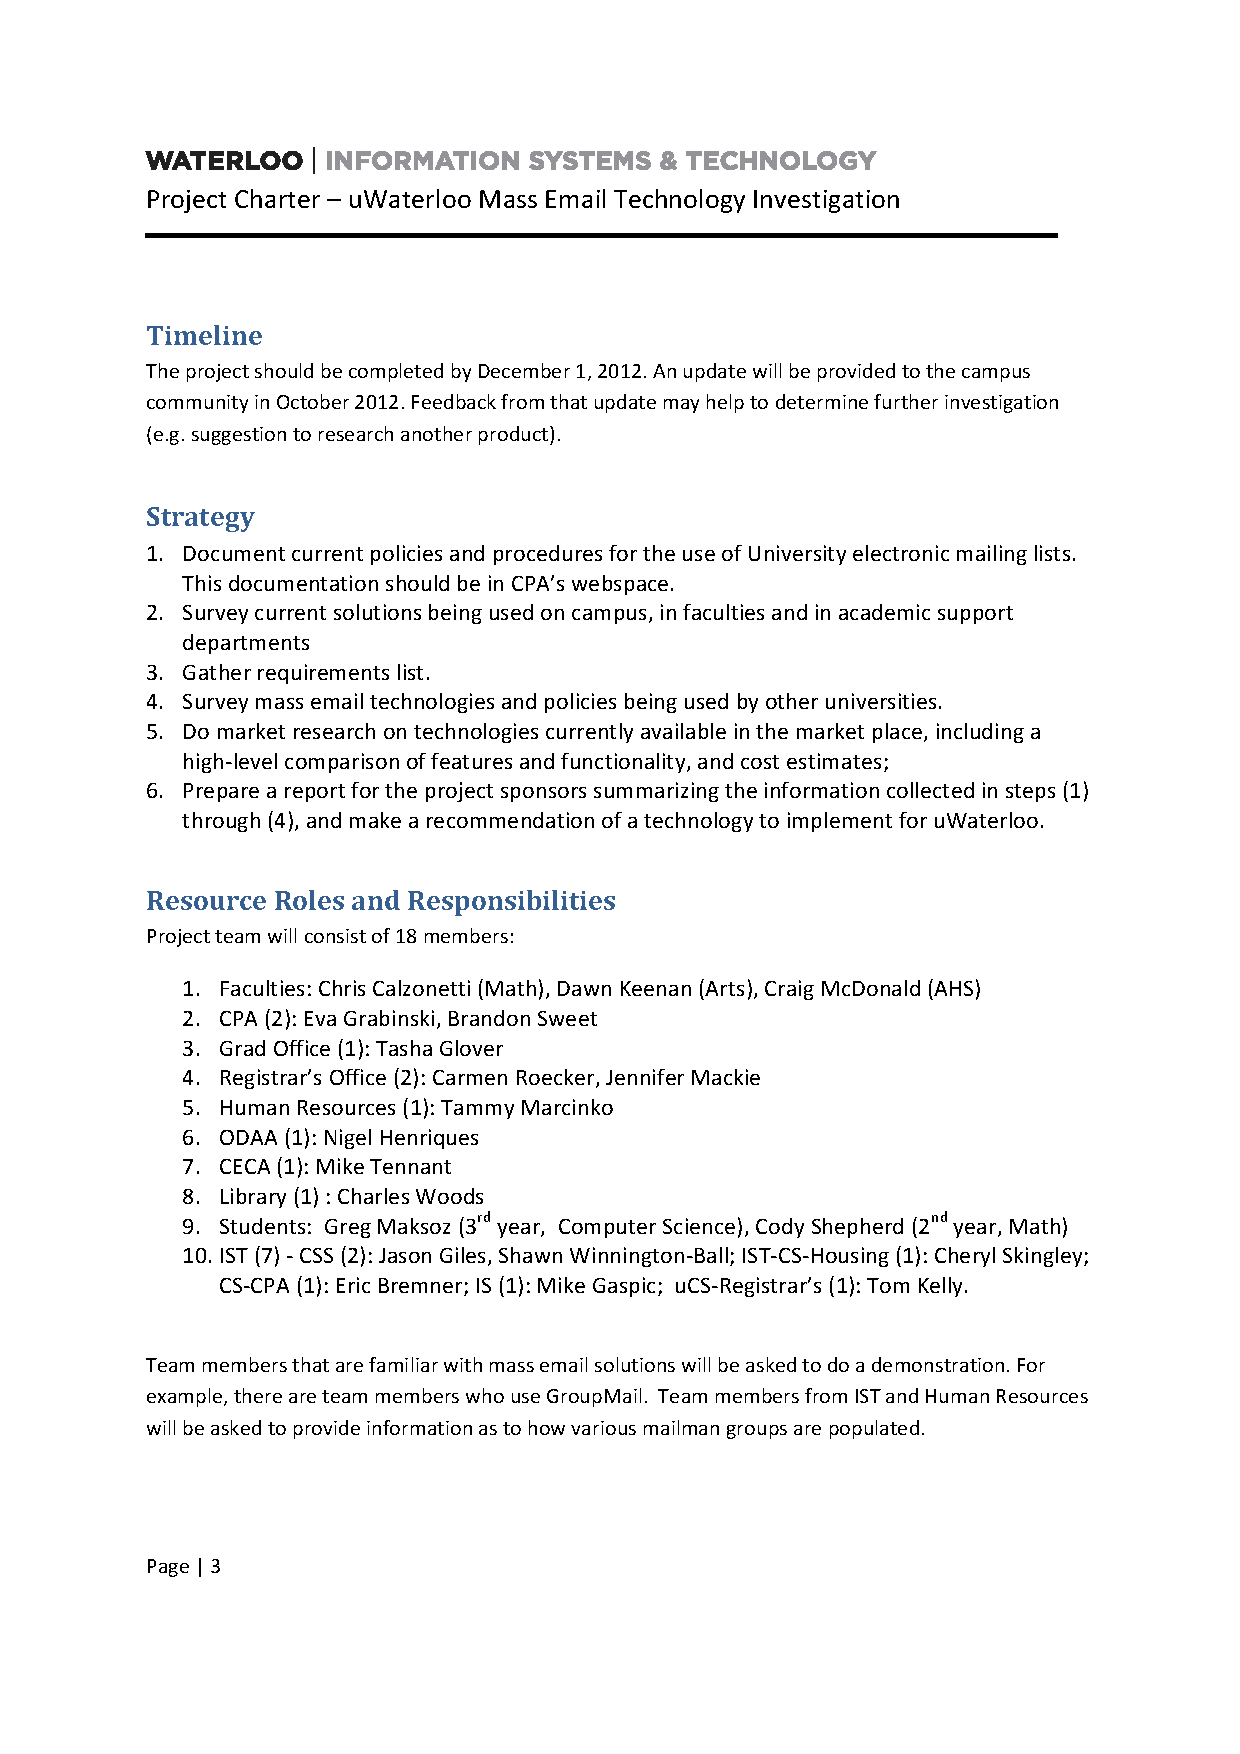
\includegraphics[scale=0.23]{pg_4}}
\end{figure}
\end{columns}
\end{frame}

%----------------------------------------------------------
\begin{frame}
\frametitle{Identifying Stakeholders}
\begin{figure}
\caption{The task of identifying stakeholders is in the \textbf{Stakeholders} knowledge area, and belongs to the \textbf{Initiating} process group.}
\vspace{-0.8cm}
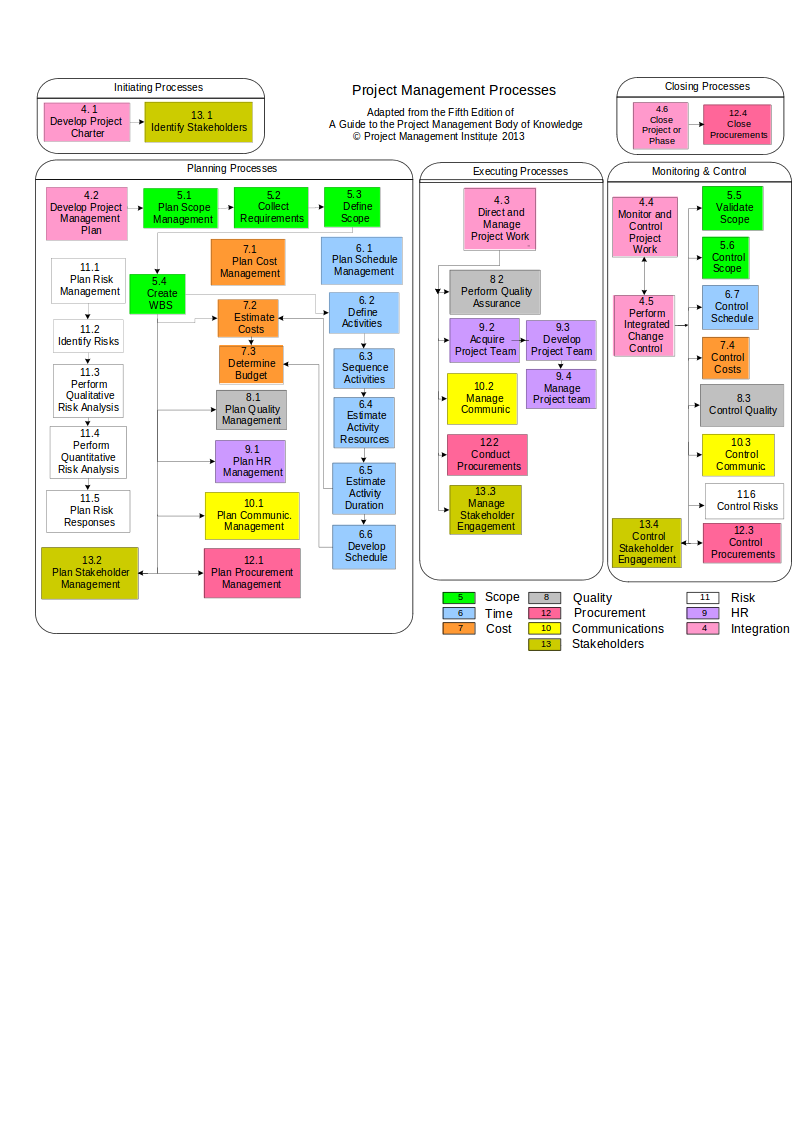
\includegraphics[scale=0.3]{mapping}
\end{figure}
\end{frame}

%----------------------------------------------------------
\begin{frame}
\frametitle{Identifying Stakeholders}
Recall that \textbf{project stakeholders}, can be positive or negative, and are the people involved in or affected by project activities. Stakeholders can be classified as \textbf{internal} of \textbf{external}:
\vspace{0.5cm}
\begin{itemize}
\item \textbf{Internal project stakeholders} generally include the project sponsor, project team, support staff, and internal customers for the project.
\item \textbf{External project stakeholders} include the project's customers (if they are external to the organisation), competitors, suppliers, and other external groups that are potentially involved in or affected by the project, such as government officials and concerned citizens.
\end{itemize}
\end{frame}

%----------------------------------------------------------
\begin{frame}
\frametitle{Identifying Stakeholders}
\begin{columns}[t]
\column{0.45\textwidth}
\begin{tcolorbox}
\textbf{Internal Stakeholders}\\

\footnotesize Can be positive or negative - generally includes:
\begin{itemize}
\item project sponsor
\item project team
\item support staff
\item internal customers for the project
\item top management
\item other functional managers
\item other project managers
\end{itemize}
\end{tcolorbox}
\column{0.45\textwidth}
\begin{tcolorbox}
\textbf{External Stakeholders}\\

\footnotesize Generally includes:
\begin{itemize}
\item project's customers (if they are external to the organisation)
\item competitors
\item suppliers
\item other external groups that are potentially involved in or affected by the project, such as government officials and concerned citizens
\end{itemize}
\end{tcolorbox}
\end{columns}
\end{frame}

%----------------------------------------------------------
\begin{frame}
\frametitle{Identifying Stakeholders}
\textbf{Using a Mindmap to Identify Stakeholders}
\begin{figure}
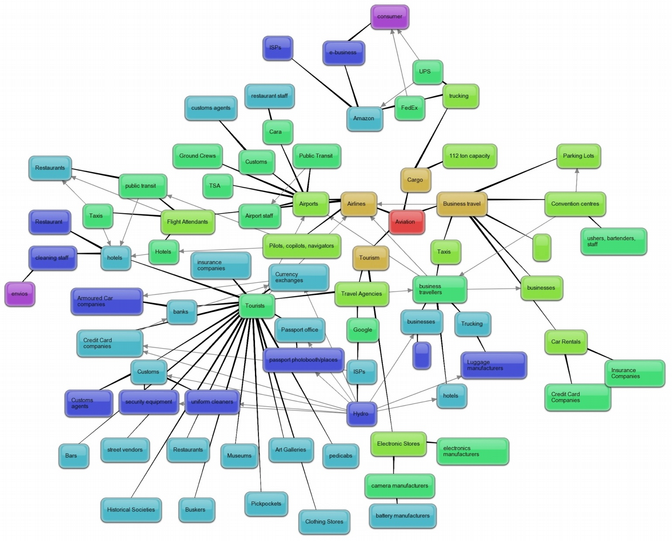
\includegraphics[scale=0.45]{mind_map_stakeholder}
\end{figure}
\end{frame}

%----------------------------------------------------------
\begin{frame}
\frametitle{Identifying Stakeholders}
\textbf{Stakeholder Register and Stakeholder Analysis}\\
\vspace{0.5cm}
The task of identifying stakeholders can be broken down into two subtasks: creating a \textbf{stakeholder register}, and performing \textbf{stakeholder analysis}.
\vspace{0.5cm}
\begin{block}{Definition: \textbf{Stakeholder Register}}
A \textbf{stakeholder register} is a document that includes details related to the identified project stakeholders - usually available to many people, so it should not include sensitive information
\end{block}
\vspace{0.2cm}
\begin{block}{Definition: \textbf{Stakeholder Analysis}}
A \textbf{stakeholder analysis} is a technique for analysing information to determine which stakeholders' interests to focus on and how to increase stakeholder support throughout the project.
\end{block}
\end{frame}

%----------------------------------------------------------
\begin{frame}
\frametitle{Identifying Stakeholders}
\textbf{Example of a Stakeholder Register}\\
\begin{figure}
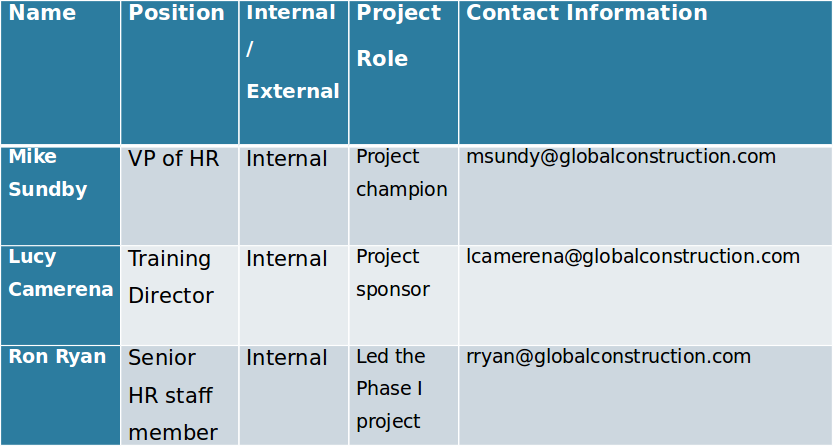
\includegraphics[scale=0.5]{stakeholder_reg}
\caption{An example of a stakeholder register. There are many different formats - try Googling \textit{Stakeholder Register Template}}
\end{figure}
\end{frame}

%----------------------------------------------------------
\begin{frame}
\frametitle{Identifying Stakeholders}
\textbf{What should a stakeholder analysis include?}
\vspace{0.5cm}
\begin{itemize}
\item Names and organisations of key stakeholders
\item Their roles on the project
\item Unique facts about each stakeholder
\item Their levels of interest in the project
\item Their influence on the project
\item Suggestions for managing relationships with each stakeholder
\end{itemize}
\end{frame}

%----------------------------------------------------------
\begin{frame}
\frametitle{Identifying Stakeholders}
\textbf{Example of a Stakeholder Analysis}
\begin{figure}
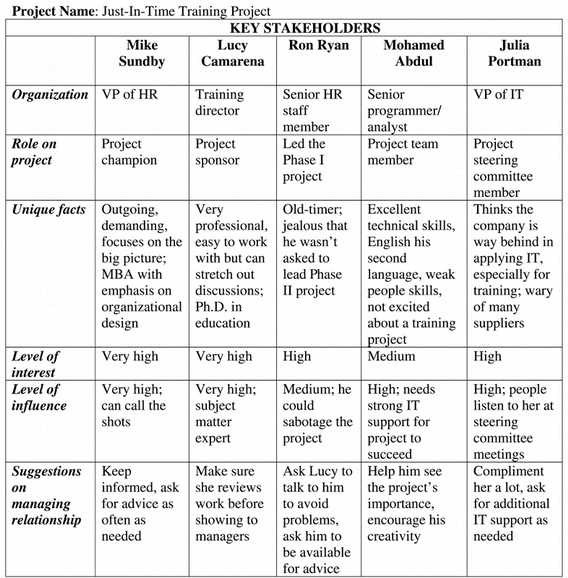
\includegraphics[scale=0.4]{stakeholder_analysis}
\caption{An example of a stakeholder analysis matrix.}
\end{figure}
\end{frame}

%----------------------------------------------------------
\begin{frame}
\frametitle{Identifying Stakeholders}
\textbf{Example of Stakeholder Analysis Power and Interest Grid}\\
\begin{figure}
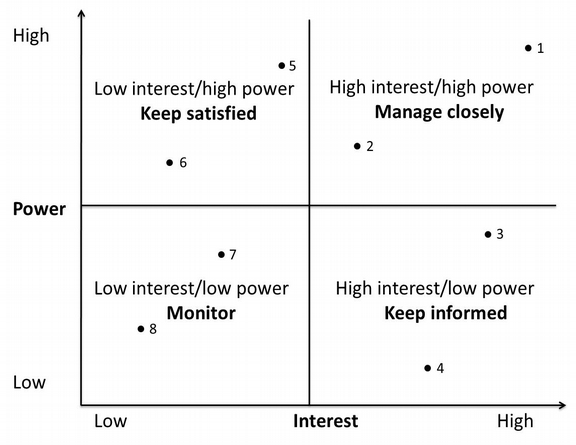
\includegraphics[scale=0.5]{stakeholder_analysis_grid}
\caption{A graph, called a stakeholder power and interest grid, can help to visually explain some of the aspects of your stakeholder analysis.}
\end{figure}
\end{frame}

%----------------------------------------------------------
\begin{frame}
\frametitle{Identifying Stakeholders}
\textbf{Categorising Engagement Levels of Stakeholders}\\
\vspace{0.5cm}
Stakeholders' level of engagement is typically identified as one of the following:
\begin{itemize}
\item \textbf{Unaware}: unaware of the project and its potential impacts on them.
\item \textbf{Resistant}: aware of the project yet resistant to change.
\item \textbf{Neutral}: aware of the project yet neither supportive nor resistant
\item \textbf{Supportive}: aware of the project and supportive of change.
\item \textbf{Leading}: aware of the project and its potential impacts and actively engaged in helping it succeed.
\end{itemize}
\end{frame}

%----------------------------------------------------------
\begin{frame}
\frametitle{Holding a Project Kickoff Meeting}
\begin{block}{Definition: \textbf{Kick-off Meeting}}
A \textbf{kick-off meeting} is a meeting held at the beginning of a project so that stakeholders can meet each other, review the goals of the project, and discuss future plans.
\end{block}

\begin{itemize}
\item Experienced project managers know that it is crucial to get projects off to a great start
\item Often \textbf{kick-off meetings} are used to get support for a project and clarify roles and responsibilities
\item The project champion should speak first and introduce the project sponsor and project manager
\item Often a fair amount of work is done to prepare for the meeting
\item Kick-off meetings are held face to face
\end{itemize}
\end{frame}

%----------------------------------------------------------
\begin{frame}
\frametitle{Holding a Project Kickoff Meeting}
\textbf{Example of a Kick-off Meeting Agenda}
\begin{figure}
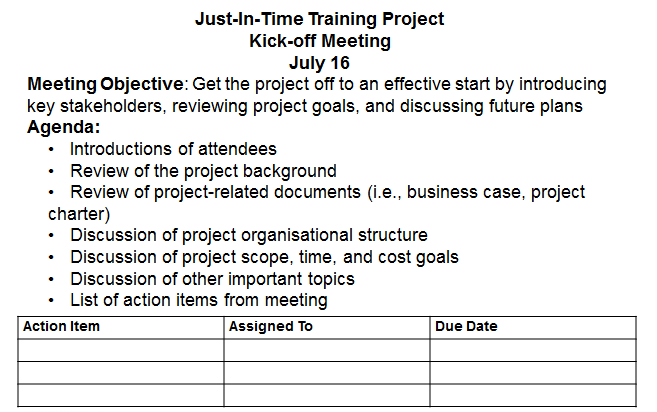
\includegraphics[scale=0.5]{kick_off}
\caption{An example of the agenda for a kick-off meeting.  There are many templates which are available on the internet - try Googling \textit{Kick-off Meeting Template}.}
\end{figure}
\end{frame}

%----------------------------------------------------------
\begin{frame}
\begin{center}
\huge The End
\end{center}
\end{frame}
\end{document} 